\documentclass[a4paper]{article}

\title{IDS projekt\,--\,1.\,časť}
\author{Adam Lazík\\
Michal Ľaš}

\usepackage[slovak]{babel}
\usepackage[left=3cm, top=3cm]{geometry}
\usepackage[utf8]{inputenc}
\usepackage[T1]{fontenc}
\usepackage{graphicx}
\usepackage{float}

\begin{document}

\maketitle

\section{Zadanie}

Zvolili sme zadanie č.~23\,--\,\textbf{Stavebná firma}.
Zadanie sme pojali ako vytvorenie interného informačného systému českej stavebnej firmy, ktorá okrem zamestatncov zamestnáva aj iné české firmy a českých živnostníkov tak, že za dohodnutú sumu využíva ich služby na rôznych zákazkách.

\section{Prípady užitia}

\begin{figure}[H]
    \centering
    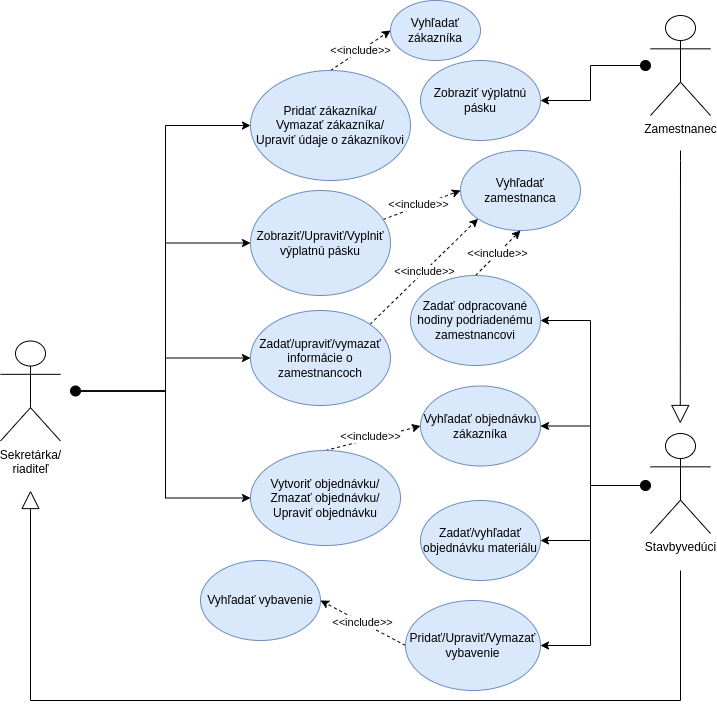
\includegraphics[width=\linewidth,height=0.55\textheight,keepaspectratio]{StavebnaFirmaUseCase.png}
    \caption{Diagram prípadov užitia}
\end{figure}

So systémom môžu manipulovať zamestnanci firmy.
Bežný zamestnanec si môže nechať zobraziť svoju výplatnú pásku za každý mesiac.

Stavbyvedúci môže navyše vyhľadať objednávky zákazníkov a objednávky materiálu, zadať informácie o novej objednávke materiálu a zadať odpracované hodiny podriadených zamestnancov.

Sekretárka môže vykonávať všetky akcie ako stavbyvedúci a navyše môže zadávať údaje o nových zamestnancoch a zákazníkoch a nové objednávky zákazníkov a vypĺňať výplatné pásky zamestnancov.
Sektretárka tiež môže všetky tieto údaje meniť pre prípad, že by pri zadávaní údajov došlo k chybe.

\section{Dátový model}

\begin{figure}[H]
    \centering
    \includegraphics[width=\linewidth,height=0.7\textheight,keepaspectratio]{StavebnaFirma.png}
    \caption{ER diagram}
\end{figure}

Informačný systém uchováva kontaktné údaje o zákazníkoch firmy.
Pre jednoznačné rozlíšenie zákazníkov je každému zákazníkovi informačným systémom vygenerované jedinečné ID.\@

IS uchováva objednávky zákazníkov.
Pri vytvorení záznamu o zákazníkovi poverenou osobou zákazník nemusí mať zadanú žiadnu objednávku.
Každá objednávka má informačným systémom vygenerované jedinečné číslo objednávky, ktoré ju identifikuje.
V objednávke uchovávame adresu, kde sa konajú stavebné práce, cenu, dátum začiatku a konca výstavby (dátum kolaudácie), stručný jednovetový popis, napr. \textbf{výstavba obytného domu}, status, napr. \textbf{v procese} alebo \textbf{dokončená}, a dátum poslednej úpravy špecifikácie.
Samotnú špecifikáciu obsahujúcu požiadavky zákazníka a detailný plán výstavby považujeme za príliš veľkú na to, aby bolo uloženie v databáze efektívne, preto sa tieto budú ukladať do súborov mimo databáze a v databázi je uložená iba  cesta k tomuto súboru.\@

Objednávky môžu vyžadovať rôzny materiál pre ich úspešné dokončenie a ku každej objednávke môže byť asociovaných niekoľko (i nula) objednávok materiálu.
Firma neobjednáva materiál bez objednavky zákazníka, preto bez tejto objednavky materiálu nemôže existovať.
Objednávka materiálu je identifikovaná číslom objednávky zákazníka, ku ktorej je objednávka materiálu viazaná, a ID objednávky materiálu, ktoré generuje informačný systém.
O objednávke materiálu systém ukladá základné informácie a číslo objednávky generované dodávateľom.
Samotný dokument o objednávke znovu považujeme za priveľký na uskladnenie v databáze a pokladáme za efektívnejšie uskladňovať tieto mimo databázy, takže v databázi je uložená iba cesta k súboru.

IS ďalej uchováva informácie o externých a interných zamestnancoch firmy.
Interných zamestnancov jednoznačne identifikuje číslo zdravotného preukazu, pretože človek pracujúci v Českej republike musí mať české zdravotné poistenie.

Okrem osobných, kontaktných a platobných údajov ďalej IS uchováva o zamestnancovi typ úväzku, ktorý je vyjadrený počtom hodín práce za pracovný deň, hodiny platenej a neplatenej dovolenky za rok plat na hodinu.

Zamestnanec môže mať nula (bežný pracovník) až n (stavbyvedúci\dots) podriadených a nula (riaditeľ) až jedného (ostatní) priameho nadriadeného.

Špeciálny prípad zamestnanca je poverený pracovník\,--\,kam spadá sekretárka, stavbyvedúci a riaditeľ\,--\,ktorý môže zadávať objednavky na materiál a  kupovať pracovné vybavenie.

Vybavenie je identifikované unikátnym ID a uchováva sa o ňom cena, druh, stav (napr. \textbf{nepoškodený} alebo \textbf{opotrebovaný}), dátum nákupu a cesta k nákupnej zmluve.

IS ukladá výplatné listiny zamestnancov za každý mesiac. Vo výplatnej listine sa nachádza počet odpracovaných hodín a celková mzda (aby sa dal spätne vypočítať hodinový plat za každý mesiac), počet hodín platenej a neplatenej dovolenky a finančné odmeny nad rámec platu získané v daný mesiac.

Na objednávkach ďalej môžu pracovať externí zamestnanci, tzn.\ firmy alebo živnostníci, ktorých objednáva stavebná firma na konkrétnu objednávku.
Externí zamestnanci sú jednoznačne identifikovaní \textbf{IČO}m a ďalej IS o nich ukladá kontaktné a platobné údaje a špecializáciu.
Externí zamestnanci kupujú materiál na vlastné náklady a preto toto nie je potrebné zaznamenávať v IS.\@

Pri každej objednávke sa zaznamenáva, ktorí interní a externí zamestnenci na nej pracujú, od kedy do kedy, a aký druh práce vykonávajú.
V prípade externých zamestnancov sa zaznamenáva aj dohodnutá cena práce.

\end{document}